\chapter{Conclusion and discussion}
\label{chap:discussion}

\section{Summary of findings}
In language after language, we find three clause types (\diis{}) that are dedicated to three speech acts (\aqrs{}). By 18 months old, children seem to be able to differentiate these clause types and associate them with their canonical speech act. To gain this ability, they need to identify the right categories of clauses (i.e.\ solve the clustering problem) and figure out what speech act they are canonically used for (i.e.\ solve the labeling problem). To solve the labeling problem, some speech act information must be available to the learner, but since there is the possibility of mismatches -- sentences used to perform speech acts that are not canonically associated with their clause types -- it is not immediately clear how useful it is for learners to be able to identify speech acts, if it is useful at all. Then, to solve the clustering problem, children surely need to pay attention to the surface morpho-syntactic features of each sentence in their input. But in the input that learners actually receive, many surface features might be absent or misleading. Again, it seems plausible that the availability of some information related to speech acts might be helpful to the learner, but this information too is potentially misleading, again due to cases where sentences are used to perform speech acts that are not canonically associated with their clause type.

This dissertation investigates how children figure out clause type categories. In particular, are the surface formal features of the sentences in the input sufficient for children to figure out the clustering of clause types? If not, is speech act information helpful for solving the clustering problem? And how might learners access such speech act information?

I addressed these questions computationally by simulating two learners, a \distlearner{} (\dlearnerabbr{}), and a \praglearner{} (\plearnerabbr{}). Both learners use the surface morpho-syntactic features of the input sentences to attempt to cluster sentences into three categories, i.e.\ to learn the clause type categories. But the \plearnerabbr{} additionally has access to some information about which speech act is performed by a sentence. I found that in English, the \dlearnerabbr{} model could identify interrogative clause but could not identify the other two clauses, but in Mandarin, this model cannot find any of the right categories. The \plearnerabbr{} model in both languages outperforms the \dlearnerabbr{}. In English, the \plearnerabbr{} model can find all three clause types; in Mandarin, the model has problem with imperative clauses. These results suggest that pragmatics is helpful, indeed crucial, to solve the clustering problem. 

\revise{Another useful source of information is prosody. With a corpus study, I found that parents do not use final rises more often with questions. But if we look at subcategories of interrogatives, polar interrogatives have more final rises than other types of speech acts and clause types, including \twh-interrogatives and declaratives. I incorporated prosodic information into the two models, but found that this information does not improve \dlearnerabbr{'s} performance. Speech act information is still necessary for learners to find the right clause type clustering. }

But if the speech act information is useful for clause type learning, how do children figure out speech act information? Given that the way we generally identify a speech act is via its clause type, there is a potentially vicious circle here -- you need to identify a sentence's clause type to infer the speech act that is being performed, but you need to be able to infer speech act information to learn to identify clause types. How do learners avoid this circularity?

One way to break this circularity is to \tit{not} think of the learning of speech acts and clause types as two processes that need to happen sequentially, but as a joint learning process. It is likely that children learn to identify speech act and clause type in tandem and mutually informative ways.

To get one step closer to understanding and evaluating this joint learning hypothesis, I first addressed the question of how much speech act information children need to identify clause types. With the \plearnerabbr{} model, I simulated the learning of clause type with various degrees of noise in the speech act information. I showed that even if children can only perceive speech act information a small proportion of the time, they can still benefit from this information, as a noisy pragmatic percept is superior to no pragmatics at all. 



I then explored what kind of non-clause type cues for speech act information are present in the input. Even if children must rely on clause type information to figure out the speech acts, they could have access to additional information that is unrelated to clause typing, but is informative for recognizing speech act type. When speakers perform speech acts, because of the conventional functions of these speech acts on the discourse, the performance might be associated with certain socio-pragmatic features. For example, because of questions' response-elicitation function, we would expect pauses after questions. With prior knowledge about the functions of communication, and expectations about what questions do, children might able to use these socio-pragmatic features to figure out this speech act. If children have such expectations, could they find anything in the input? 

I explored three cues that could potentially differentiate questions from other speech acts: pauses, and direct eye gaze. I found that parents tend to pause longer after questions, and attend to the child more when asking questions. Therefore it is in principle plausible that there are some socio-pragmatic features that children can use, in addition to their growing knowledge of clause types to infer the speech act category of an utterance. This little bit of information about speech act could then be used to provide enough pragmatic information that the child needs in order to get the clause type clusters identified accurately.

\section{The pragmatic syntactic bootstrapping hypothesis}

When examined separately, the learning of clause types and the learning of speech acts share many similarities. 
%The learning of clause types seem to parallel with the learning problems typically associated with the semantic bootstrapping hypothesis, and the learning of speech act categories seem to parallel to some degree to the problems addressed by the syntactic bootstrapping hypothesis. Let's look at them one by one. 


The clause type categories are abstract formal features of a sentence related to a variety of surface forms, none of which is obligatorily present and many of which can occur in sentences with a different clause-type feature. While in principle the surface formal features could be sufficient, this dissertation showed that they in fact fall short. To compensate for this insufficiency, learners can use the speech act information -- which is systematically related to clause types -- to learn to identify clause types and which surface features are relevant for clause typing.

%Leaving aside the nature of speech act categories for now, but they are also not directly observable from the input, same as clause types, and need to be inferred. 
Speech acts are abstract pragmatic/semantic/conceptual categories. As we have seen in Chapter~\ref{chap:eng-sp}, speech act categories are related to a variety of human behaviors (e.g. pauses and eye gaze), none of which are obligatorily present (you don't \emph{need} to pause after a question) and many of which can occur when performing other speech act categories. While I showed that the features are correlated with the use of questions, it is likely that the learners use the clause type information --- which is systematically related to speech acts --- to inform how they infer speech act types.

In both learning processes, one source of information could bridge the gap between the learners' input and the abstract category they need to acquire, because of the robust correlation between the major clause types and the major speech act types across languages. 

But as I have discussed throughout this dissertation, when we put these two learning processes together, our first impression is that there is a chicken-and-egg problem: the learner needs speech act information to learn clause types, but they also needs clause types to learn speech act information. To break this vicious cycle, \hypos{} proposes that the learner has to learn the two in tandem, with sentential force connecting the two categories:

\begin{exe}\ex\label{ex:prag-syn-hypo}
\tbf{The \hypos{}}:\\
\revise{
Children learn to identify the sentential force of a sentence by observing the speech acts that the sentence is used to perform on the one hand, and observing the syntactic clause types in tandem and mutually informative ways: children learn to identify clause types by tracking formal regularities in conjunction with their growing knowledge of speech acts and its associated social pragmatic cues; similarly, they identify speech acts by tracking social pragmatic cues in conjunction with their growing understanding of the syntax of clause types. }
\end{exe} 

\begin{comment}


\bex{}
\ex
\begin{tikzpicture}[level distance=60pt]
\tikzset{every tree node/.style={align=center,anchor=north, font=\scriptsize}}
%}}
\tikzset{level 1/.style={level distance=35pt}}
\tikzset{level 2/.style={sibling distance=35pt}}
%\tikzset{level 3/.style={sibling distance=-6pt}}
%\tikzset{level 4+/.style={sibling distance=-6pt}}
\Tree
[. {Sentential force} 
	[. {Clause type features\\ ([\textpm int, imp])} 
		[. {Surface formal features} ]
		[. {Prosodic features} ]
	]
	[. {Speech act categories \\
	\aqrs{}} 
		
		[. {Prosodic features} ]
		[. {Social pragmatic features} ]
	]
]

\end{tikzpicture}
\eex
\end{comment}


In this dissertation, I have established (a) that the learning of clause types does not require perfect speech act information; thus, it is possible that children learn clause type information while still trying to figure out the speech act information. And, (b) that there are social pragmatic cues associated with the use of the speech act of questioning. So if a child is equipped with a theory of what questions do, in addition to an innate knowledge that there are speech act categories that are associated with clause types, they could potentially find the signals they need.

In future work, I plan to test the feasibility of the speech act bootstrapping hypothesis computationally.



\subsection{\revise{Determining the role of prosody}}

\revise{As discussed in Chapter~\ref{chap:background}, the role of prosody for clause typing might be complicated, which affects how learners might use prosody. Considering the fact that some languages do not use prosodic features for clause typing, it is possible that children do not have a priori knowledge that prosodic features are informative for clause type categorization.  }

\revise{If children do not assume prosody informs clause typing, Italian- and Portuguese-acquiring children might need to learn the connection between prosody and clause typing, in addition to learning clause type and speech act categories. But it is also possible that children do not need to learn this connection at all. Since children assume prosody informs speech acts, and that speech acts are informative of clause typing, prosodic information could indirectly help the learning of clause type categories. }

\revise{It is also possible that children come to the learning task assuming that prosody \tit{does} inform clause typing. For children learning languages like Vata, where prosody is irrelevant for clause typing in their language, the input might be such that this connection is simply uninformative. Thus, assuming the connection between clause typing and prosody would not make any difference for the learning the clause type categories. To test this possibility, we need to look at the input to Vata-acquiring children, and see if assuming the link between prosody and clause type would hinder children from learning the right clause type clustering. }

\revise{Another possibility is that instead of directly informing clause type and/or speech act categories, the learners need to combine prosodic features with some morpho-syntactic features, so that they can find the distinction between polar interrogatives and declaratives. }


\revise{In Chapter~\ref{chap:prosody}, I adopted the second strategy, as the speech act information is assumed to be either inaccessible or observable in our current models. As we have seen, prosody does not improve the performance of the \distlearner. But if speech act categories also need to be learned, then we could test how different ways of utilizing prosodic information could influence the learning of clause types and speech acts. Our model also only utilizes one prosodic features, final rise. It's possible that if the model has access to more prosodic features, its performance could improve. }

\revise{This leads us to another complication related to prosody, namely languages use different prosodic features for clause typing, and many of them are not correlated with a rising F0 at the end. For example, Akan's breathy termination in fact results in the lowering of F0. Therefore, instead of having a built-in knowledge of the form ``final rise $\sim$ questionhood," children might need to learn to which prosodic features are associated with which speech act/clause type clusters, the same way that they need to learn which morpho-syntactic features go with which clause type cluster.}

\revise{In my simulations in Chapter~\ref{chap:prosody}, we only considered one feature, final rise. In the future, I plan to include more features to better approximate the learning process.  }


\subsection{\revise{From matrix to embedded clauses}}

\revise{In this dissertation, I primarily focus on the clause type and speech act of the matrix clauses. This is mostly due to the pragmatical reason that infants at 18 months old might not have figured out embedded clauses yet. The question then is, can we extend our current model to embedded clauses?}

\revise{While the \hypos{} discussed in the previous section is in parallel with the \hypos{} proposed by \textcite{hacquardlidz2018} for the learning of attitude verbs that can embed clauses, it is not straightforward to extend our current discussion with matrix clauses to the embedded clauses. While pragmatics can help learners to figure out matrix clause types, embedded clauses do not have their own speech act information. Additionally, many morpho-syntactic features associated with matrix clauses disappears in embedded contexts. For example, embedded interrogatives no longer have subject-auxiliary inversion:}
\bex{}
Ann knows whether it is raining.
\eex

\revise{However, it is likely that the speech act of the whole utterance still aligns with the clause type of the embedded clause. For example, the speaker is likely asking ``is it raining'' when using \ref{ex:conclusion:embed}. If this is the case, then speech act information might continue helping learners to identify the clause type categories of embedded clauses.}

\bex{ex:conclusion:embed}
I wonder whether it's raining.
\eex

\revise{I plan to expand the corpus to include more embedded clauses, and annotate additional features for embedded clauses (e.g. children might have figured out what are complementizers at this point, so we no longer need to lump \tit{whether} with other Unknown Function Items). We can then test what kind of information is needed for children to figure out which surface feature goes with which clause types in embedded contexts.   } 

\begin{comment}

 
 
 
Figure~\ref{fg:model} shows the graphical model. 
  
\begin{figure}[H]
\centering
\begin{tikzpicture}[
  node distance= 0.8cm and 0.8cm,
  classnode/.style={draw,ellipse,text width=0.3cm,align=center},
  enode/.style={draw,ellipse,text width=0.2cm,align=center},
  obsnode/.style={draw,ellipse,text width=0.3cm,align=center, fill=black!30}
]
\node[classnode] (a) {$A$};
\node[obsnode, below right=of a] (p) {$P$};
\node[classnode, below left =of a] (c) {$C$};
\node[obsnode, below left=of c] (s) {$S$};
\node[obsnode, below right =of c] (f) {$F$};
%\node[enode, left=of c] (e) {$e$};
\path (a) edge[-latex] (p)
(a) edge[-latex] (c)
(c) edge[-latex] (s)
(c) edge[-latex] (f)
(a) edge[-latex] (f)
;
\end{tikzpicture}
\caption{Graphical Model}\label{fg:model}
\end{figure}

The question is then whether it is possible for a learner to use the expected social pragmatic cues to initially identify questions in their input, and use this speech act information to bootstrap the process of learning to identify the surface properties of interrogative clauses. The proposed model will (i) track the prosodic and pragmatic features of each utterance and infer the speech act that would generate these features; (ii) using knowledge of prosodic and syntactic features of each sentence, the model will be able to identify the clause type that would generate these features; and (iii) speech and clause type categories will influence each other. The advantage of such a learner is that it can exploit pragmatics to identify clause type indirectly via identifying the speech act, and exploit syntax to identify speech act indirectly via identifying the clause type. 


\revise{}

In our situation, the learners need to figure out two abstract categories, the clause types and the speech acts information, and the =two categories need to be learned in tandem. 

\tbf{The \hypos{}} (alternative):\\
Children learn to identify the sentential force of a sentence by observing the speech acts that the sentence is used to perform on the one hand, and observing the syntactic clause types in tandem and mutually informative ways: children learn to identify clause types by tracking formal regularities in conjunction with their growing knowledge of speech acts and its associated social pragmatic cues; similarly, they identify speech acts by tracking social pragmatic cues in conjunction with their growing understanding of the syntax of clause types. 

because of the systematic mapping between the three major clause types and the three major speech acts, 
The semantic bootstrapping hypothesis states that:
\begin{quote}
[T]he child uses the presence of \tit{semantic} entities such as ``thing,'' ``causal agent,'' ``true in past'' and ``predicate-argument relation'' to infer that the input contains tokens of the corresponding syntactic substantive universals such as \tit{noun}, \tit{subject}, \tit{auxiliary}, \tit{dominates} and so on.\\
\hspace*{\fill} \cite[407]{pinker1987} 
\end{quote}
\end{comment}
%%%%

%When putting these two together, it first appears that we might have a chicken-and-egg problem: 

